\documentclass[10pt,a4paper,titlepage,oneside]{book}
\usepackage[utf8]{inputenc}
\usepackage[czech]{babel}

\usepackage{amsfonts}
\usepackage[IL2]{fontenc} 
\usepackage{graphicx}
\usepackage{epstopdf}
\usepackage{fancyhdr}
\usepackage{mathtools}
\usepackage{float}
\fancyhf{}

\newcommand{\itab}[1]{\hspace{0em}\rlap{#1}}
\newcommand{\tab}[1]{\hspace{.2\textwidth}\rlap{#1}}

\usepackage[top=2.5cm, bottom=2.5cm, left=2.5cm, right=2.5cm]{geometry}
%\usepackage[a4paper]{geometry}

\providecommand{\e}[1]{\ensuremath{\times 10^{#1}}}



\begin{document}
\title{Realizace experimentů pro odhad parametrů dynamického modelu látky}
\author{Michal Neoral}
\date{\today{}}
\maketitle

\thispagestyle{fancy}

\part*{Návod na pořízení dat}


\section*{Úvod}

Tato práce je součástí mezinárodního projektu CloPeMa (Clothes Perception Manipulation). Tento dokument obsahuje postup a popis sběru dat pro tvorbu dynamického modelu textilie.\\
\\
CLoPeMa je tříletý výzkumný projekt zaměřený na výzkum a vývoj v oblasti autonomního snímání a manipulace s textiliemi a oděvy. Systém je postaven na základě operačního systému ROS (Robot Operating System) a jako hlavní programovací jazyky jsou vybrány C++, Python a Java [1].\\
\\
Cílem projektu je prohloubit vědecké a praktické znalosti v této oblasti. Významnou části projektu je řešení problému integrace a fúze dat z oblasti kamerového snímání, rozpoznávání, učení, mechaniky a robotiky [1].\\
\\
Předpokládá se významný přínos projektu v oblasti průmyslové automatizace a robotického 3D snímání pro technologicky náročné aplikace. Výzkum vedoucí k těmto výsledkům byl podporován Evropskou unií v Sedmém Rámcovém Programu (FP7/2012-2014) grantem číslo 288553 CloPeMa [1].\\
\\

\section*{Způsob pořízení dat}
Ramena robota najedou za pomocí skriptu \verb|collect_data.py| (viz. kapitola Pořízení dat) do polohy, kdy rameno r1 je v takové pozici, ve které je rovina snímače kamery kolmá na rovinu podlahy a zároveň rotace kamery, kolem osy kolmé na rovinu snímače, je nulová.\\
\\
Rameno r2 nabývá dvou základních poloh. Poloha jedna je pro odfiltrování pozadí snímků (viz. kapitola \textit{Načtení dat pro další zpracování}). V této poloze je rameno zcela mimo snímaný úsek obrazu.\\
\\ 
Druhou polohou ramene r2 je poloha, ve které je připraveno k provedení experimentu. Rameno je v takové poloze, aby textilie do něj zachycená byla v takové výšce, aby byla kamerou uchycenou na ramenu r1 zachycen ten kus textilie, který nás zajímá nejvíce. Zároveň musí být v takové pozici, aby, při pohybu charakteristického pro experiment (dále jen „třepání“), mohl hýbat jak ve směru dopředu/dozadu, tak i vlevo/vpravo. Volené směry jsou brány vzhledem k rovině snímače kamery, tedy dopředu/dozadu je pohyb k/od roviny snímače kamery apod. (viz. Obrázek 1).\\
\\
\begin{figure}[H]
	\centering  	
  	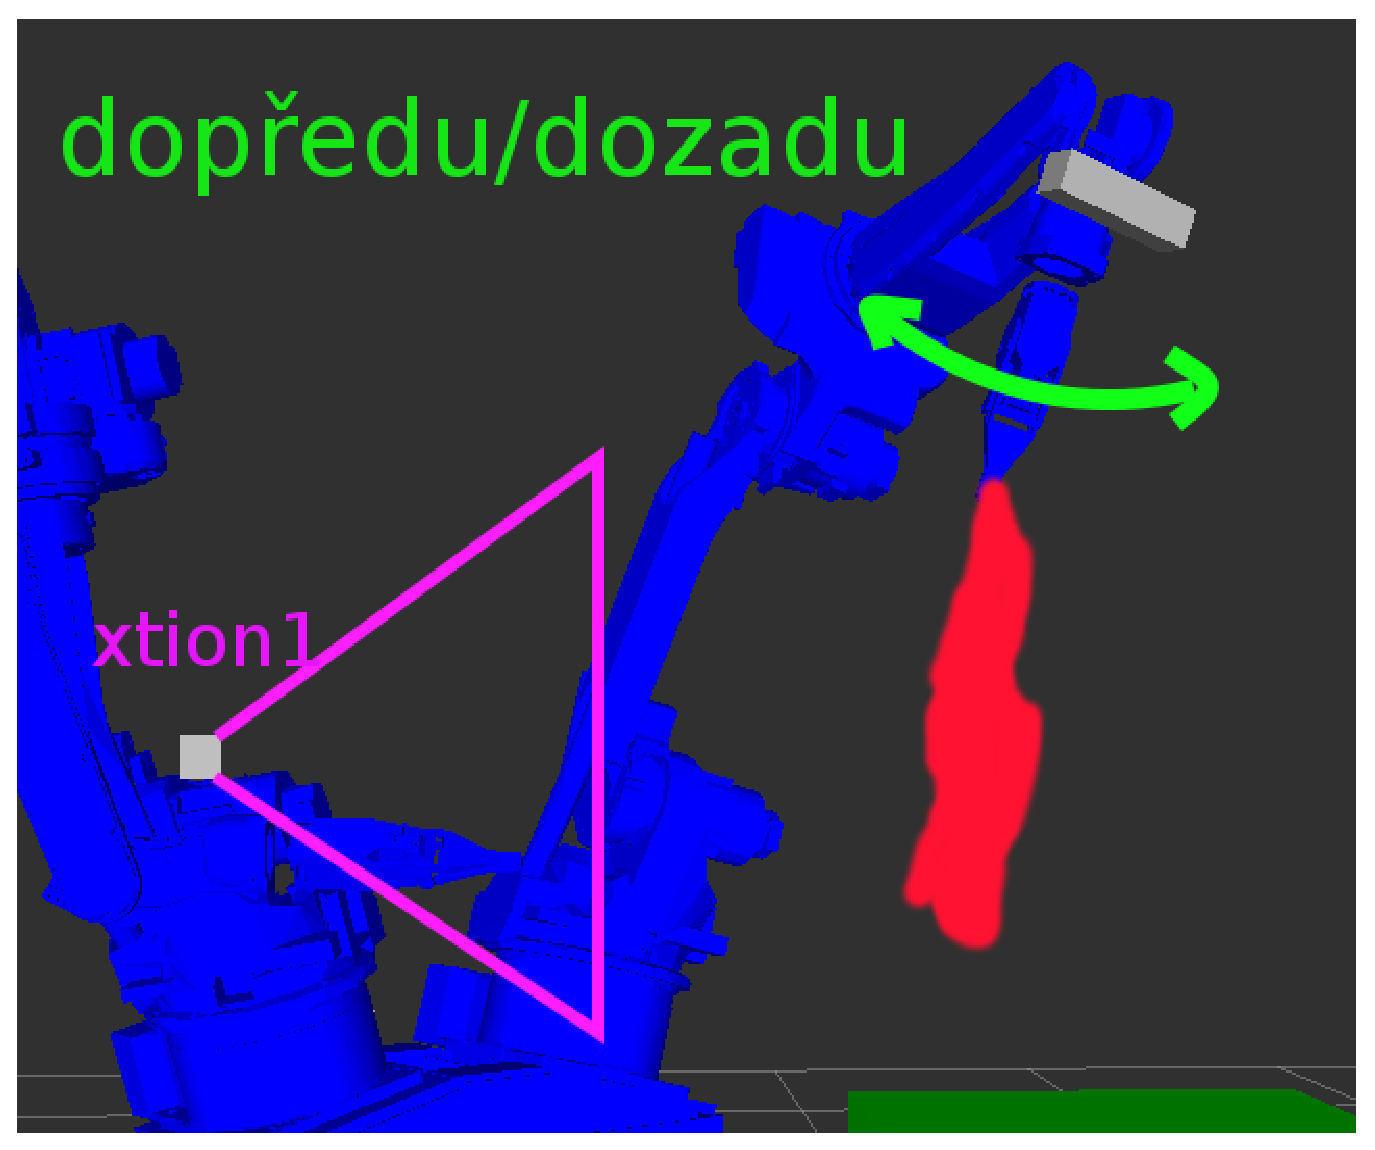
\includegraphics[height=7cm]{pictures/obrazek1.eps}
  	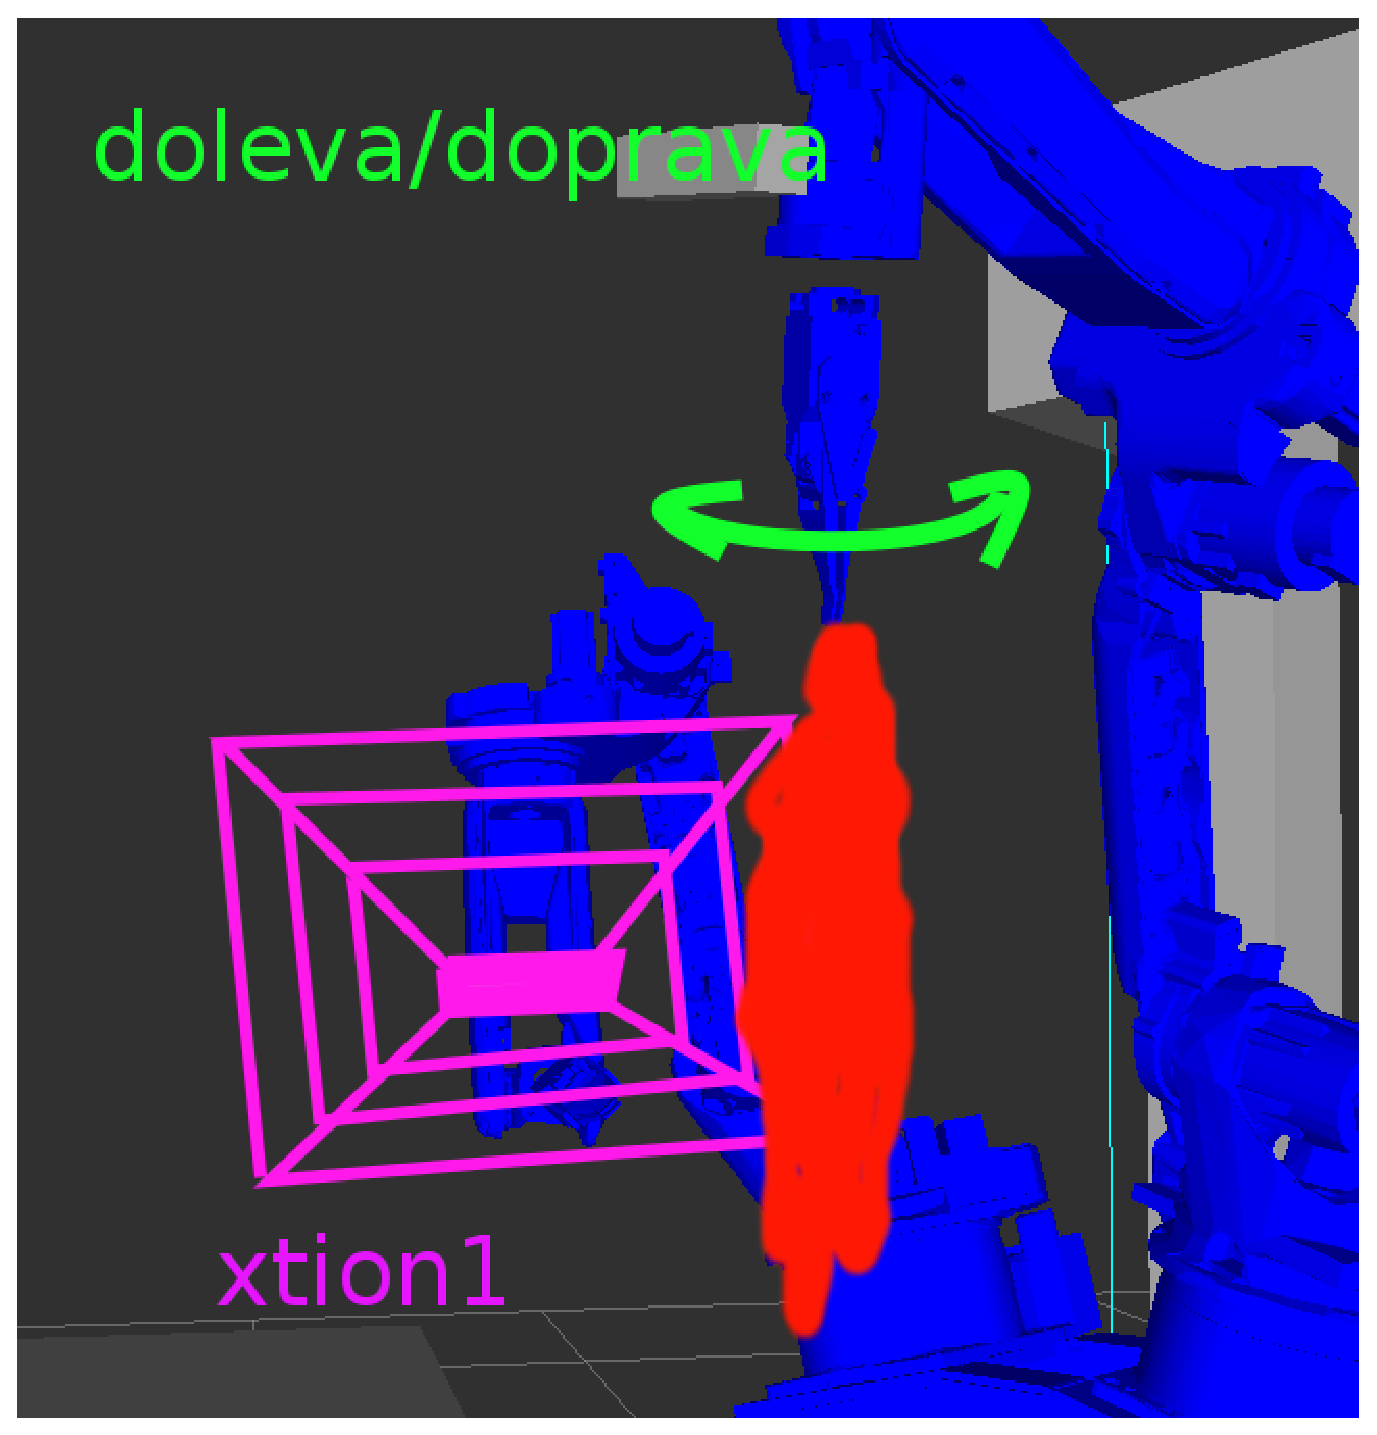
\includegraphics[height=7cm]{pictures/obrazek2.eps}
  	\caption{Nastínění pohybů chapadla s textilií.}
  	\label{fig:obrazek1}
\end{figure}
Externí osa (osa č.: 13) je otočena tak, aby v pozadí snímané textilie bylo co nejméně rušivých předmětů. Nejlépe jednobarevný rovný povrch.
\\
\\
Jak již bylo naznačeno v předchozím odstavci je třeba nasnímat obraz pro odfiltrování pozadí.\\
\\
Do chapadla je uchycena textilie. Rameno manipulátoru poté provede pohyb – zatřepe s látkou. Nejdříve ve směru k dopředu/dozadu, následně se chapadlo otočí a provede se pohyb vlevo/vpravo.\\
\\
Po skončení snímání je možné vyměnit látku a postup zopakovat.\\
\\

\section*{Pořízení dat}
\subsection*{Předpoklady:}

\begin{itemize}
  \item Nainstalovaný ROS Hydro a balíčky Clopema:
  \begin{itemize} 
  
  	\item \verb|http://clopema.felk.cvut.cz/redmine/projects/clopema/wiki/CloPeMa_Packages|
  \end{itemize}
  
  \item Stáhnutý archív se zdrojovými kódy:
  \begin{itemize}
  	\item \verb|git clone https://github.com/michalneoral/clopema_collect_model_data.git|
  \end{itemize}
  
  \item V balíčku \verb|clopema_collect_model_data| ve složce src upraven scritp \verb|local_options.py| pro místní nastavení počítače.
  \begin{itemize}
  	\item \verb|pcglocate| pro umístění složky se zdrojovými kódy
  	\item \verb|savefolder| umístění složky, kam se budou ukládat získaná data.
  \end{itemize}  
\end{itemize}


\subsection*{Postup spouštění:}

\begin{itemize}
  \item Spustíme robota: 
  \begin{itemize} 
  
  	\item \verb|roslaunch clopema_launch start_robot.launch|
  \end{itemize}
  
  \item Spustíme kameru na ramenu r1:
  \begin{itemize}
  	\item \verb|roslaunch clopema_launch xtion1.launch|
  \end{itemize}
  
  \item Poté, co se tyto věci úspěšně spustí můžeme spustit vlastní skript pro sběr dat:
  \begin{itemize}
  	\item \verb|rosrun clopema_collect_model_data collect_data.py|
  \end{itemize}
  
  \item Program je ovládán z příkazové řádky:
  
\end{itemize}

\begin{figure}[H]
	\centering  	
  	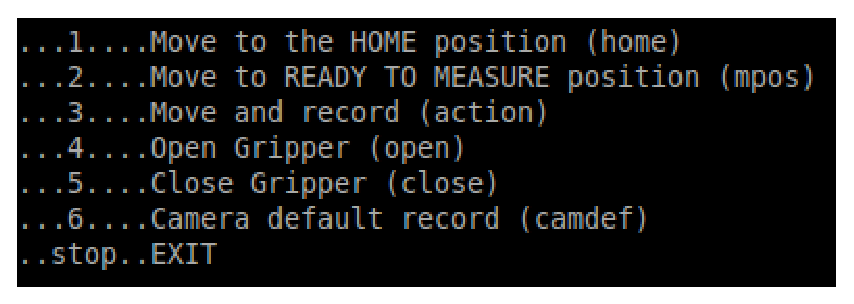
\includegraphics[scale=0.6]{pictures/obrazek3.eps}
  	\caption{Náhled menu skriptu}
  	\label{fig:obrazek3}
\end{figure}

\subsection*{Postup pro nasnímání obrazu pro odfiltrování pozadí:}
\begin{enumerate}
  \item Využijeme funkci \textbf{(6)} – \textit{Camera default record}.
\end{enumerate}

\subsection*{Postup pořízení dat – manuální vkládání textilie:}
\begin{enumerate}
  \item Umístíme robota do polohy, ve které je připraven k měření \textbf{(2)} - \textit{Move to READY TO MEASURE position}.
  \item Otevřeme chapadlo \textbf{(4)} – \textit{Open Gripper}.
  \item Zavřeme chapadlo \textbf{(5)} – \textit{Close Gripper}. Po stisknutí máme 5 vteřin pro vložení textilie do chapadla než se chapadlo sevře.
  \item Po sevření chapadlo ustoupíme do bezpečné vzdálenosti od robota.
  \item Zahájíme měření a záznám \textbf{(3)} - \textit{Move and record}.
  \item Budeme vyzvání k pojmenování souboru. Doporučuji nazývat souboru názvem textilie, případně i pořadovým číslem.
  \item Po schválení názvu souboru bude provedeno měření způsobem, který je popsán v předchozí kapitole \textit{(Způsob pořízení dat)}.
  \item Postup 2. až 7. můžeme opakovat pro další měření.
  \item Před ukončením programu můžeme pomocí \textbf{(1)} umístit robota do výchozí polohy.
  \item Program ukončíme pomocí \textbf{(exit)}.
\end{enumerate}

\section*{Uložení dat}
Data se ukládají pomocí rosbag ve formátu “.bag“ do předem určené složky uložené v souboru local\_options.py (\verb|path_to_workspace/clopema_collect\_model_data/src/local_options.py|).\\
\\

Z důvodu úspory místa a kapacity přenosového kanálu jsou zaznamenány pouze témata (topic), která jsou uložena v souboru topics.txt  (\verb|path_to_workspace/clopema_collect_model_data/matlab/topics.txt|). Pro tento experiment jsem vybral tyto témata (topic):\\
\\
\indent \indent \indent \verb|/joint_states| \\
\indent \indent \indent \verb|/tf| \\
\indent \indent \indent \verb|/xtion1/depth/camera\_info| \\
\indent \indent \indent \verb|/xtion1/depth_registered/camera_info| \\
\indent \indent \indent \verb|/xtion1/projector/camera\_info| \\
\indent \indent \indent \verb|/xtion1/rgb/camera_info| \\
\indent \indent \indent \verb|/xtion1/depth/image_raw| \\
\indent \indent \indent \verb|/xtion1/rgb/image_raw |\\
\indent \indent \indent \verb|/xtion1/depth/disparity |\\
\indent \indent \indent \verb|/xtion1/depth/points|\\
\\

Seznam témat je možné libovolně měnit. Zaznamenáno je 7 vteřin dat.\\
\\
Zaznamenané soubory jsou ve tvaru: \verb|name_speed_AX.bag|

\begin{itemize}
\item \itab{name}  \tab{vámi zadaný název}
\item \itab{speed} \tab{nastavená rychlost manipulátoru} 
\item \itab{A} \tab{osa, kterou bylo vykonáno "třepání" - \textit{R} nebo \textit{B}}
\item \itab{X}  \tab{číslo souboru s tématy, která jsou zaznamenána}  
\end{itemize}

\section*{Načtení dat pro další zpracování}
\subsection*{Předpoklady:}
\begin{itemize}
   \item Stahnutý archív se zdrojovými kódy
  \begin{itemize}
  	\item \verb|git clone https://github.com/michalneoral/clopema_collect_model_data.git|
  \end{itemize}
  
  \item Nainstalovaný Matlab (odzkoušeno ve verzi 2012b i 2013a).
  \item Nainstalovaný toolbox pro matlab „rosbag“ a přidána cesta pro tento toolbox. Toolbox je dostupný i s návodem k instalaci na adrese:
  \begin{itemize}
     \item \verb|https://github.com/bcharrow/matlab_rosbag|
  \end{itemize}
  \item Nacházet se ve složce se zdrojovými kódy pro Matlab.
  \item Soubor \verb|topics.txt| musí být stejný jako v době nahrávání .bag souboru.
\end{itemize}

V proměnné \verb|path_to_bag_files| je potřeba mít uloženou cestu k uloženým .bag souborům s daty a v proměnné \verb|topics| je načten soubor \verb|topics.txt| s názvy požadovaných témat (viz. \verb|startup.m|).\\
\\
Načítání souborů spustíte příkazem \verb|loader|, který vypíše soubory v zadané složce (\verb|path_to_bag_files|) a nechá vybrat soubor pro načtení do Matlabu a vypíše informace o souboru. Pro správnou funkci tohoto skriptu je třeba mít nasnímáno a uloženo „čisté“ pozadí (popsáno v kapitole \textit{Návod na pořízení dat}).\\
\\
Tento příkaz dále spustí skript \verb|reader|, který převede soubor .bag na čitelnější strukturu \verb|msgs| (provede rovněž i pro „čisté“ pozadí \verb|msgs_bag|) a předpřipravý RGB obrázek „čistého“ pozadí - \verb|rgb_back| (takto předpřipravené data lze zobrazovat pomocí \verb|imshow(data)| nebo \verb|image(data)| jako 2D obrazy). \\
\\
Příkaz loader dále předpřipraví data z RGB i hloubkové kamery do zásobníku obrazu \verb|front|, která je seřazená tak, aby si obrazy odpovídaly časovými značkami. První řádek obsahuje původní RGB obrazy, druhý řádek obsahuje RGB obrazy s odfiltrovaným pozadím a třetí řádek obsahuje data z hloubkové kamery v metrech.
Spolu se strukturou \verb|front| se tvoří i struktura \verb|queue|, jenž v obsahuje tyto údaje:

$$\begin{bmatrix}
\verb|pořad. číslo hloubkového snímku| & \verb|čas od začátku měření| & \verb|pořad. číslo tématu v msgs| \\
  \verb|pořad. číslo rgb snímku| & \verb|časový rozdíl mezi snímky| & \verb|pořad. číslo tématu v msgs|
\end{bmatrix} $$\\
\\

Další pokračování existuje, ale je potřeba ho konzultovat.
%\section*{Provedení experimentu}

\section*{Aktuální verze tohoto návodu}
\verb|https://github.com/michalneoral/collect_data_documentation/|\\
\verb|raw/master/manual_collect_data(cze).pdf|\\

\begin{thebibliography}{NEO}    
  \bibitem[1]{homesim} Neovision:
    \emph{Industrial Vision System} [online]. [cit. 2013-11-12].\\
    Dostupné z: \verb|http://www.neovision.cz/cz/sols/clopema.html|
    
\end{thebibliography}

\end{document}

